% ============================================================
%  Нейросетевая аппроксимация и решение обратных задач
%  Курс: Продвинутые методы машинного обучения — МФТИ
%
%  Компиляция:
%    pdflatex -interaction=nonstopmode -output-directory=../.latex_cache ml_course.tex
% ============================================================

\documentclass[11pt, aspectratio=169]{beamer}

% ── Кириллица (Arch Linux / TeX Live) ────────────────────────
\usepackage[T2A]{fontenc}
\usepackage[utf8]{inputenc}
\usepackage[english, russian]{babel}
\usepackage{tempora}

% ── Тема ─────────────────────────────────────────────────────
\usetheme{Madrid}
\usecolortheme{whale}
\usefonttheme{professionalfonts}
\setbeamertemplate{navigation symbols}{}

% ── Пакеты ───────────────────────────────────────────────────
\usepackage{amsmath, amssymb, bm}
\usepackage{booktabs}
\usepackage{xcolor}
\usepackage{tikz}
\usepackage{pgfplots}
\pgfplotsset{compat=1.18}
\usepackage{graphicx}
\usepackage{array}

% ── Цвета ────────────────────────────────────────────────────
\definecolor{mlblue}{RGB}{30, 80, 162}
\definecolor{mlorange}{RGB}{214, 100, 40}
\definecolor{mlgreen}{RGB}{40, 160, 80}

\setbeamercolor{frametitle}{bg=mlblue, fg=white}
\setbeamercolor{alerted text}{fg=mlorange}
\setbeamercolor{block title}{bg=mlblue!85, fg=white}
\setbeamercolor{block body}{bg=mlblue!8}
\setbeamercolor{block title alerted}{bg=mlorange!85, fg=white}
\setbeamercolor{block body alerted}{bg=mlorange!8}
\setbeamercolor{block title example}{bg=mlgreen!75, fg=white}
\setbeamercolor{block body example}{bg=mlgreen!8}

% ── Метаданные ───────────────────────────────────────────────
\title[Deep Calibration]{%
  Нейросетевая аппроксимация и решение обратных задач\\[-2pt]
  в стохастических моделях}
\subtitle{\textit{«Deep learning volatility...»}\\[-1pt]
  Horvath, Muguruza \& Tomas, \textit{Quantitative Finance}}
\author[Бирюков Н.]{Бирюков Никита}
\institute[МФТИ]{МФТИ}
\date[18.05.2026]{Продвинутые методы МО \quad 18.05.2026}

% ─────────────────────────────────────────────────────────────
\begin{document}
% ─────────────────────────────────────────────────────────────

% ══════════════════════════════════════════════════════════════
% Слайд 1 — Титульный
% ══════════════════════════════════════════════════════════════
\begin{frame}[plain, noframenumbering]
  \vspace{0.5em}
  {\centering
    {\large\bfseries\color{mlblue} Нейросетевая аппроксимация и решение обратных задач}\\[0.3em]
    {\normalsize\color{mlblue} в стохастических моделях (Deep Calibration)}\\[0.6em]
    {\small\itshape «Deep learning volatility...»\\[-1pt]
     Horvath, Muguruza \& Tomas, \textit{Quantitative Finance}}\\[1.2em]
    {\color{mlblue}\rule{0.65\textwidth}{0.4pt}}\\[0.8em]
    \begin{tabular}{rl}
      \textbf{Студент:} & Бирюков Никита \\[0.2em]
      \textbf{Тема диплома:} & Применение методов глубокого обучения \\[-1pt]
                              & для оценки и калибровки деривативов \\[0.2em]
      \textbf{Курс:} & Продвинутые методы машинного обучения \\[0.2em]
      \textbf{Дата:} & 18.05.2026 \\
    \end{tabular}
  }
\end{frame}

% ══════════════════════════════════════════════════════════════
% Слайд 2 — Введение
% ══════════════════════════════════════════════════════════════
\begin{frame}[shrink=5]{Введение: вычислительное «бутылочное горлышко»}
  \begin{columns}[T]
    \begin{column}{0.52\textwidth}
      \textbf{Проблема — решение обратной задачи:}
      \begin{itemize}\small
        \item Сложная генеративная модель
              $f:\boldsymbol\theta\!\mapsto\!\mathbf{y}$
              (симуляция Монте-Карло).
        \item \textbf{Обратная задача}: дан $\mathbf{y}^*$,
              найти $\boldsymbol\theta^*$ методом оптимизации.
        \item Каждый вызов $f$ стоит \alert{10--120 с}; оптимизатор
              требует тысячи итераций.
        \item Нет аналитического Якобиана
              $\Rightarrow$ конечные разности.
      \end{itemize}

      \smallskip
      \textbf{Актуальность:}
      \begin{itemize}\small
        \item Real-time системы — жёсткое ограничение $<\!100$ мс.
        \item \textbf{Surrogate Modeling} переносит вычисления
              на офлайн-этап.
      \end{itemize}
    \end{column}

    \begin{column}{0.45\textwidth}
      \begin{block}{Цель исследования}
        \small
        End-to-end ML-пайплайн на \textbf{PyTorch}:
        \medskip
        \begin{enumerate}
          \item \textbf{Офлайн:} обучить суррогат
                $\mathcal{N}_w\!\approx\!f$.
          \item \textbf{Онлайн:} оптимизация поверх
                замороженной $\mathcal{N}_w$,
                Якобиан — через Autograd.
        \end{enumerate}
        \medskip
        Ожидаемое ускорение: $\mathbf{>\!1000\times}$
      \end{block}
      \medskip
      {\small\itshape
       «Once trained, the surrogate makes calibration\\
        essentially instantaneous.»\\
        \hfill--- Horvath et al.\ (2019)}
    \end{column}
  \end{columns}
\end{frame}

% ══════════════════════════════════════════════════════════════
% Слайд 3 — Обзор статьи
% ══════════════════════════════════════════════════════════════
\begin{frame}[shrink=5]{Обзор статьи: двухфазная архитектура}
  \begin{columns}[T]
    \begin{column}{0.50\textwidth}
      \textbf{Главный вклад} (Horvath et al., 2019):
      \medskip
      \begin{enumerate}\small
        \item \textbf{Forward Pass (офлайн)} — обучить MLP-суррогат:
              \[
                \mathcal{N}_w:\mathbb{R}^5\!\to\!\mathbb{R}^{88}
                \;(\text{MLP }4{\times}30,\;\text{ELU})
              \]
        \item \textbf{Backward Pass (онлайн)} — оптимизатор
              поверх замороженной $\mathcal{N}_w$:
              \[
                \boldsymbol\theta^*=\arg\min_{\boldsymbol\theta}
                \|\mathcal{N}_w(\boldsymbol\theta)-\mathbf{y}^*\|^2
              \]
      \end{enumerate}

      \medskip
      \begin{block}{Результаты статьи}
        \small
        \begin{tabular}{@{}ll@{}}
          Ускорение & $>10\,000\times$ vs.\ MC \\
          Точность  & на уровне числ.\ методов \\
          Якобиан   & Autograd (бесплатно) \\
        \end{tabular}
      \end{block}
    \end{column}

    \begin{column}{0.47\textwidth}
      \textbf{Схема пайплайна:}
      \medskip
      \begin{center}
      \begin{tikzpicture}[
        box/.style={rectangle, rounded corners=3pt,
                    minimum width=2.2cm, minimum height=0.75cm,
                    align=center, font=\scriptsize, draw},
        arr/.style={->, thick},
        lbl/.style={font=\bfseries\scriptsize},
      ]
        \node[lbl, color=mlblue]   at (-0.1, 2.8) {ОФЛАЙН};
        \node[box, draw=mlblue, fill=mlblue!10] (data) at (0, 1.9)
              {Синтетика\\$(\boldsymbol\theta,\mathbf{y})$};
        \node[box, draw=mlblue, fill=mlblue!10] (nn)   at (0, 0.8)
              {MLP $\mathcal{N}_w$};
        \draw[arr, color=mlblue] (data)--(nn) node[midway,right,font=\tiny]{обучение};

        \node[lbl, color=mlorange] at (3.2, 2.8) {ОНЛАЙН};
        \node[box, draw=mlorange, fill=mlorange!10] (obs) at (3.1, 1.9)
              {Наблюдение $\mathbf{y}^*$};
        \node[box, draw=mlorange, fill=mlorange!10] (opt) at (3.1, 0.8)
              {L-BFGS-B};
        \node[box, draw=mlgreen,  fill=mlgreen!10]  (res) at (3.1,-0.2)
              {$\hat{\boldsymbol\theta}^*$};
        \draw[arr, color=mlorange] (obs)--(opt);
        \draw[arr, color=mlorange] (opt)--(res);
        \draw[->, dashed, color=mlblue] (nn.east)--++(0.35,0)
              |- (opt.west) node[near end,above,font=\tiny]{$\nabla\mathcal{N}_w$};
      \end{tikzpicture}
      \end{center}
    \end{column}
  \end{columns}
\end{frame}

% ══════════════════════════════════════════════════════════════
% Слайд 4 — Предлагаемые улучшения
% ══════════════════════════════════════════════════════════════
\begin{frame}[shrink=8]{Предлагаемые улучшения}
  \begin{columns}[T]

    % ── Левая колонка ─────────────────────────────────────────
    \begin{column}{0.45\textwidth}
      \textbf{1. $C^2$-гладкая активация ELU}\\[0.2em]
      \small
      Проблема ReLU: $f''_{\text{ReLU}}\!\equiv\!0$
      $\Rightarrow$ Гессиан нулевой.
      \[
        f_{\text{ELU}}(x)=\begin{cases}x,& x>0\\ e^x-1,& x\le0\end{cases}
      \]
      \begin{exampleblock}{\small Доказательство}
        \scriptsize
        $\|H_\text{ELU}\|_F=1.039 \gg \|H_\text{ReLU}\|_F=0$\\
        ELU сохраняет ненулевой Гессиан через Autograd.
      \end{exampleblock}

      \medskip
      \textbf{3. Total Variance $W = y^2\!\cdot T$}\\[0.2em]
      \small Суррогат предсказывает $W$ вместо $y$:
      \begin{itemize}\scriptsize
        \item Устраняет пики при малых $T$.
        \item Условие монотонности $\partial W/\partial T\!\ge\!0$
              линейно и всегда корректно.
        \item Сглаживает loss-ландшафт.
      \end{itemize}
    \end{column}

    % ── Правая колонка ────────────────────────────────────────
    \begin{column}{0.52\textwidth}
      \textbf{2. Physics-Informed Soft Constraints}\\[0.2em]
      \small
      Штрафы за нарушение структурных свойств добавляются в Loss:
      \[
        \mathcal{L}
          =\underbrace{\|\mathcal{N}_w-\mathbf{y}^*\|^2}_{\text{MSE}}
          +\underbrace{\ell_{\text{mono}}}_{\substack{\text{монотон-}\\\text{ность}}}
          +\underbrace{\ell_{\text{conv}}}_{\substack{\text{выпук-}\\\text{лость}}}
          +\underbrace{\ell_F}_{\substack{\text{жёсткий}\\\text{барьер}}}
      \]

      \begin{alertblock}{\small Три ограничения}
        \scriptsize
        \begin{tabular}{@{}ll@{}}
          $\ell_F$: жёсткий барьер & $\lambda_F=10^3$ \\
          $\ell_{\text{mono}}$: монотонность ($\partial W/\partial T\ge0$) & $\lambda=10^{-4}$ \\
          $\ell_{\text{conv}}$: выпуклость ($\partial^2 y/\partial K^2\ge0$) & $\lambda=10^{-4}$ \\
        \end{tabular}\\[0.3em]
        Все слагаемые дифференцируемы через Autograd.
      \end{alertblock}

      \medskip
      \begin{block}{\small Итог улучшений}
        \scriptsize
        \begin{tabular}{@{}ll@{}}
          Нарушений монотонности (тест) & \textbf{0 / 77} \\
          $\|H_\text{ELU}\|_F$          & \textbf{1.039} \\
          Val RMSE ($W$-пространство)   & \textbf{0.0876} \\
        \end{tabular}
      \end{block}
    \end{column}
  \end{columns}
\end{frame}

% ══════════════════════════════════════════════════════════════
% Слайд 5 — Результаты и анализ
% ══════════════════════════════════════════════════════════════
\begin{frame}[shrink=5]{Результаты и анализ}
  \begin{columns}[T]
    \begin{column}{0.50\textwidth}
      \textbf{Сетап:}
      \begin{itemize}\small
        \item PyTorch, Adam + ReduceLROnPlateau
        \item 100\,000 сэмплов (Latin Hypercube Sampling)
        \item MLP: Input(5) $\!\to\!$
              [Linear $\to$ ELU $\to$ Dropout(0.1)]$\times$4
              $\!\to\!$ Linear(88); \; 5\,698 параметров
      \end{itemize}

      \medskip
      \begin{block}{Метрики}
        \small
        \begin{tabular}{@{}lr@{}}
          \toprule
          Метрика & Значение \\ \midrule
          RMSE суррогата ($W$-пространство) & \textbf{0.0876} \\
          Время решения обратной задачи     & \textbf{47--135 мс} \\
          Нарушений монотонности (тест)     & \textbf{0 / 77} \\
          Сходимость L-BFGS-B               & 100\% \\
          Ускорение vs.\ Монте-Карло        & $\approx\mathbf{1600\times}$ \\
          \bottomrule
        \end{tabular}
      \end{block}
    \end{column}

    \begin{column}{0.47\textwidth}
      \textbf{Якобиан и Гессиан (Autograd):}
      \medskip
      \begin{center}\small
      \begin{tabular}{@{}lrr@{}}
        \toprule
        Параметр & $\partial\bar y/\partial\theta_i$
                 & $\partial^2\bar y/\partial\theta_i^2$ \\ \midrule
        $\theta_1$ & $+0.211$ & $-0.040$ \\
        $\theta_2$ & $+0.012$ & $+0.010$ \\
        $\theta_3$ & $-0.176$ & $-0.185$ \\
        $\theta_4$ & {\color{mlorange}$+1.694$} & $-0.309$ \\
        $\theta_5$ & $+0.786$ & $-0.883$ \\
        \bottomrule
      \end{tabular}
      \end{center}

      \medskip
      \begin{alertblock}{Слабая ко-идентификация (ill-posed)}
        \small Обнаружена при малых $\theta_5$: несколько
        наборов параметров дают схожий выход $\mathbf{y}$.\\
        Теоретически предсказуемо; подтверждает
        корректность пайплайна.
      \end{alertblock}
    \end{column}
  \end{columns}
\end{frame}

% ══════════════════════════════════════════════════════════════
% Слайд 6 — Демо
% ══════════════════════════════════════════════════════════════
\begin{frame}[shrink=8]{Демонстрация: интерактивный дашборд на Streamlit}
  \begin{columns}[T]
    \begin{column}{0.50\textwidth}
      \textbf{Сценарий:} микросервис real-time решения
      обратных задач.\\[0.3em]
      \textbf{Пайплайн дашборда:}
      \begin{enumerate}\small
        \item Генерация зашумлённых данных ($+1\%$ шум)
        \item Восстановление скрытых параметров ($<\!150$ мс)
        \item 3D-визуализация: целевая vs.\ восстановленная поверхность
        \item MC Dropout: $\pm2\sigma$ байесовские интервалы
        \item LSTM: прогноз по 10-дневной истории
      \end{enumerate}

      \medskip
      \textbf{Планы развития:}
      \begin{itemize}\small
        \item \textbf{Дифференциальная эволюция (DE)} для
              ухода от локальных минимумов.
        \item Normalizing Flows для полного байесовского
              инференса.
      \end{itemize}
    \end{column}

    \begin{column}{0.47\textwidth}
      \begin{center}
        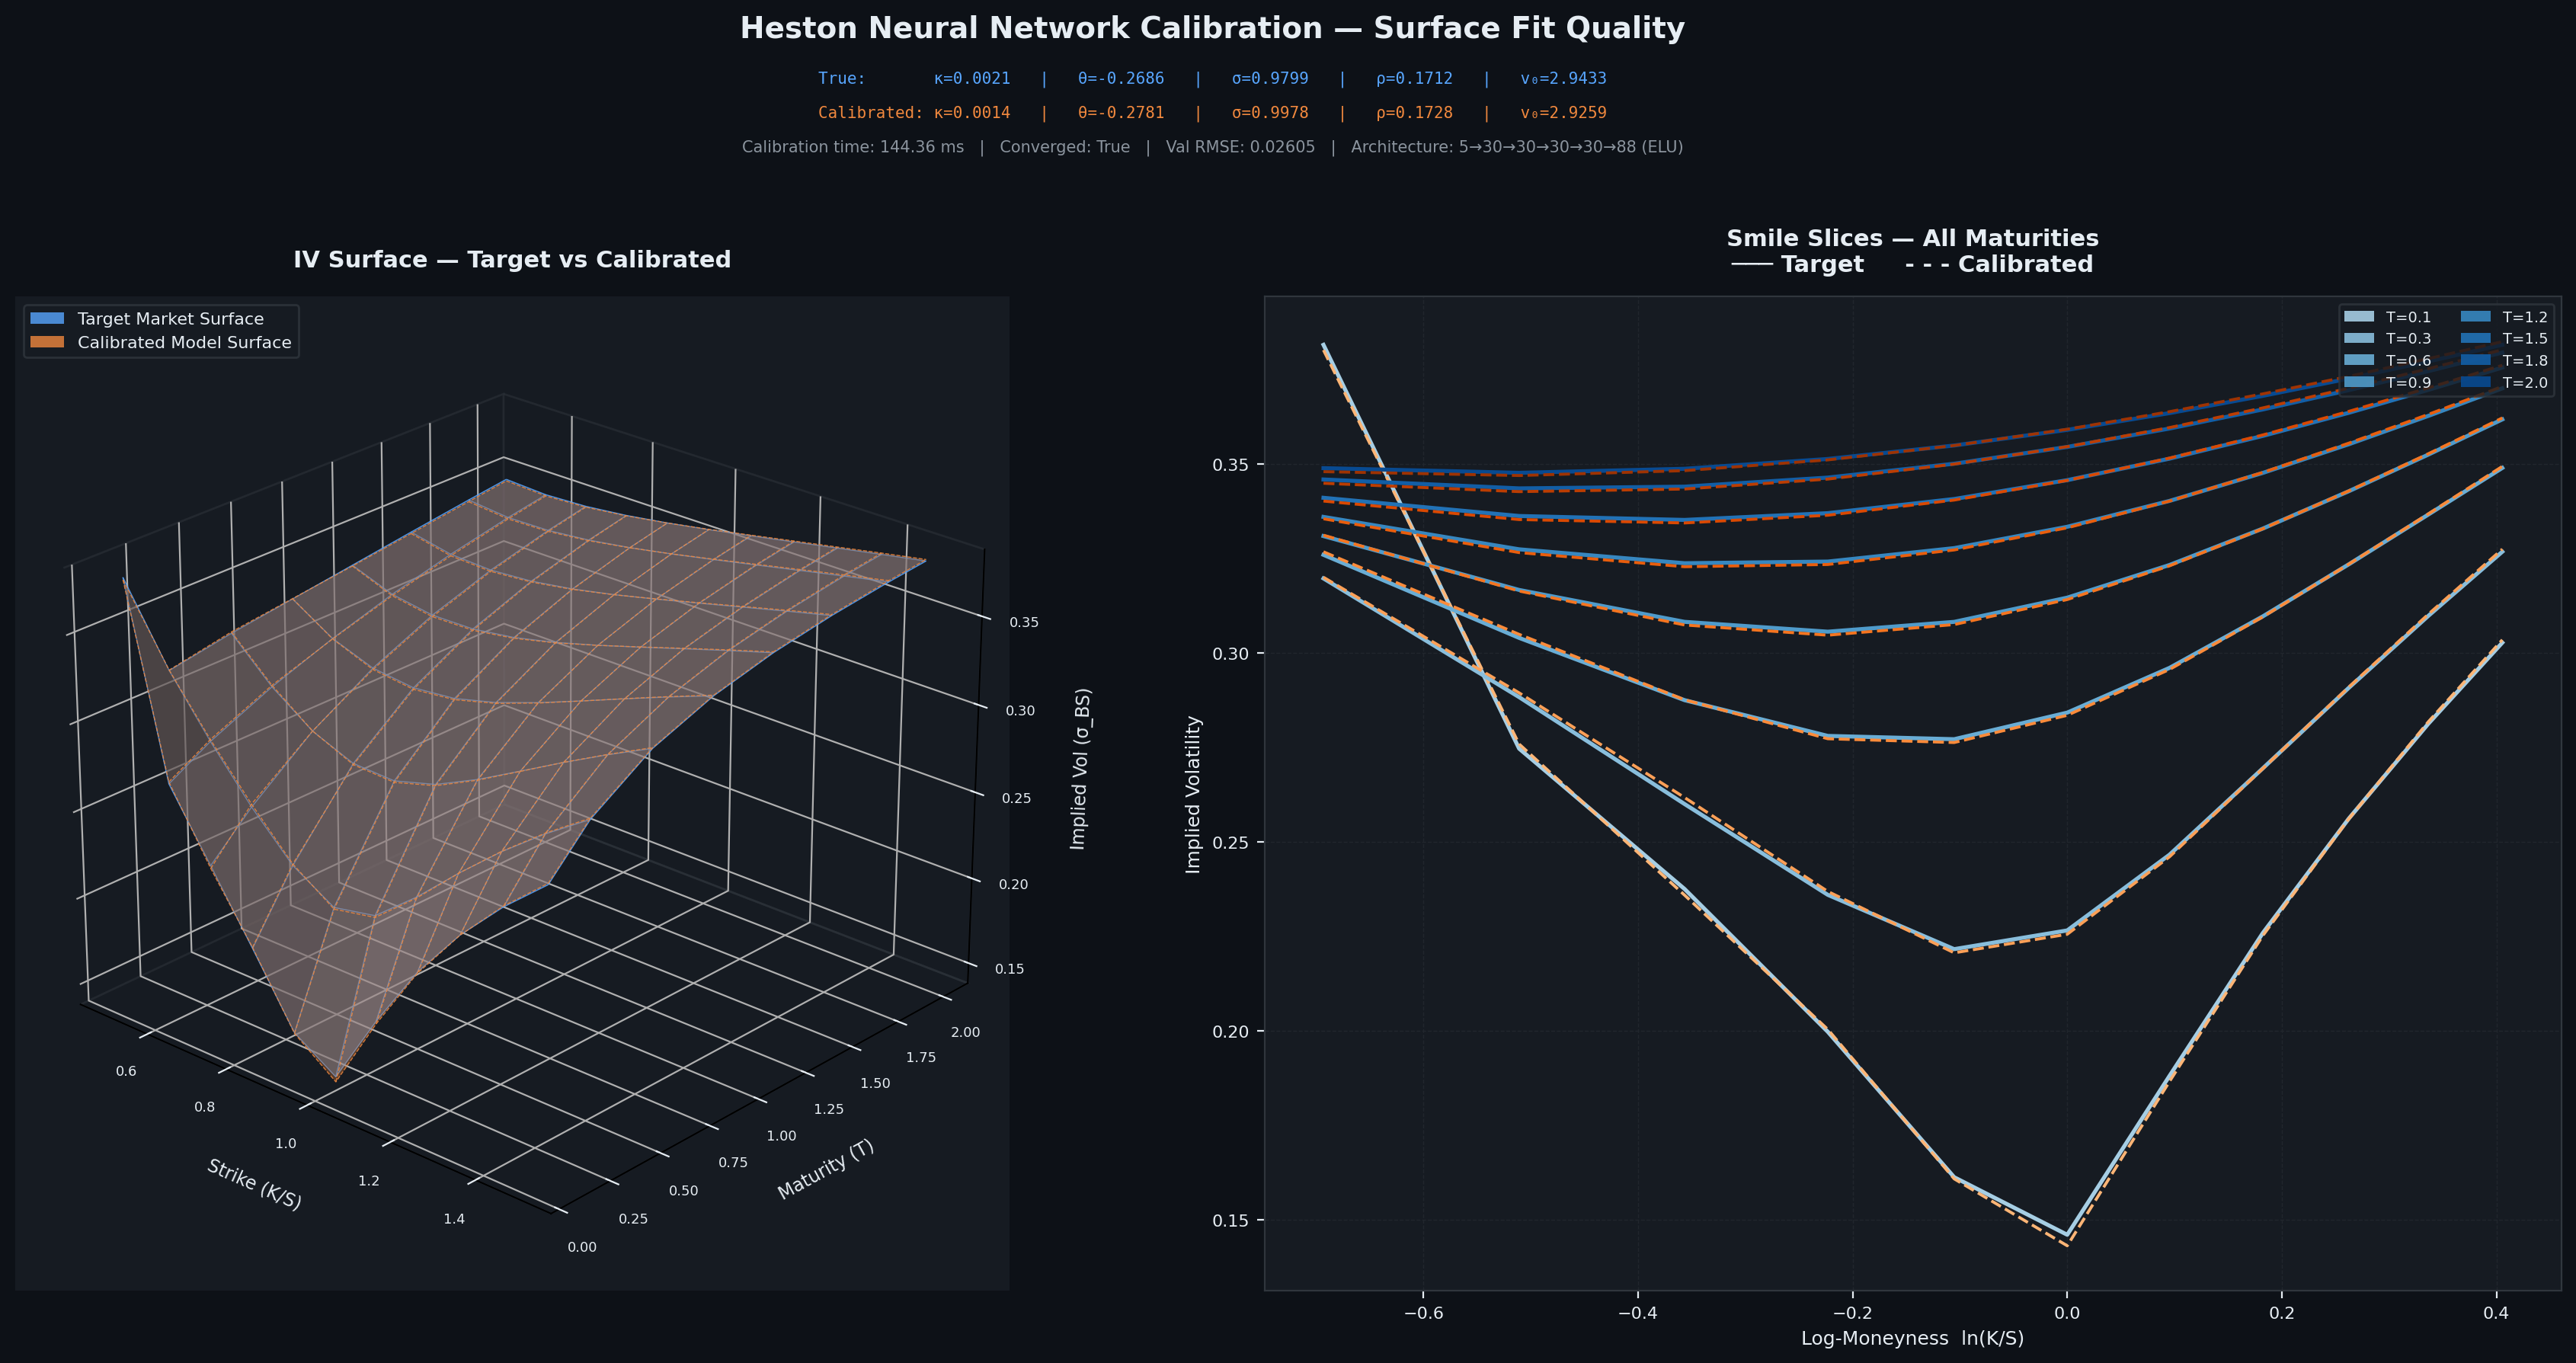
\includegraphics[width=\textwidth, height=0.38\textheight,
          keepaspectratio]{../../images/generated/surface_fit.png}\\
        {\tiny Синий --- целевая; Красный --- восстановленная}
      \end{center}

      \medskip
      \begin{exampleblock}{Отзывы коллег-ML-инженеров}
        \scriptsize
        \textit{«Отличное использование Autograd для Гессиана
        суррогата — неожиданно чисто!»}\\[0.25em]
        \textit{«Идея бесплатных байесовских интервалов
        через MC Dropout без смены архитектуры — элегантно.»}\\[0.25em]
        \textit{«Впечатляет, что LSTM обучается на синтетике
        (OU) и обобщается на реальную динамику.»}
      \end{exampleblock}
    \end{column}
  \end{columns}
\end{frame}

\end{document}
